 
\documentclass[conference]{IEEEtran}
% \IEEEoverridecommandlockouts
% The preceding line is only needed to identify funding in the first footnote. If that is unneeded, please comment it out.
\usepackage{cite}
\usepackage{hyperref}
\usepackage{amsmath,amssymb,amsfonts}
\usepackage{algorithmic}
\usepackage{graphicx}
\usepackage{textcomp}
\usepackage{xcolor}
\usepackage{tablefootnote}

\def\BibTeX{{\rm B\kern-.05em{\sc i\kern-.025em b}\kern-.08em
    T\kern-.1667em\lower.7ex\hbox{E}\kern-.125emX}}

\begin{document}

\title{Forecasting S\&P BSE SENSEX and \\ S\&P-500 Indices Using Autoregressive Integrated Moving Average (ARIMA) Model and Prophet Library.\\
	% {\footnotesize \textsuperscript{*}Note: Sub-titles are not captured in Xplore and should not be used}
	% \thanks{Identify applicable funding agency here. If none, delete this.}
}

\author{\IEEEauthorblockN{Suraj Prakash Sharma}
	\IEEEauthorblockA{\textit{M.Tech Data Science} \\
		\textit{Amrita School of Engineering, Bengaluru}\\
	Sharmasurajofficial@gmail.com}
	
	\iffalse
	\and
	\IEEEauthorblockN{2\textsuperscript{nd} Given Name Surname}
	\IEEEauthorblockA{\textit{dept. name of organization (of Aff.)} \\
		\textit{name of organization (of Aff.)}\\
		City, Country \\
	email address or ORCID}
	\and
	\IEEEauthorblockN{3\textsuperscript{rd} Given Name Surname}
	\IEEEauthorblockA{\textit{dept. name of organization (of Aff.)} \\
		\textit{name of organization (of Aff.)}\\
		City, Country \\
	email address or ORCID}
	\and
	\IEEEauthorblockN{4\textsuperscript{th} Given Name Surname}
	\IEEEauthorblockA{\textit{dept. name of organization (of Aff.)} \\
		\textit{name of organization (of Aff.)}\\
		City, Country \\
	email address or ORCID}
	\and
	\IEEEauthorblockN{5\textsuperscript{th} Given Name Surname}
	\IEEEauthorblockA{\textit{dept. name of organization (of Aff.)} \\
		\textit{name of organization (of Aff.)}\\
		City, Country \\
	email address or ORCID}
	\and
	\IEEEauthorblockN{6\textsuperscript{th} Given Name Surname}
	\IEEEauthorblockA{\textit{dept. name of organization (of Aff.)} \\
		\textit{name of organization (of Aff.)}\\
		City, Country \\
	email address or ORCID}
	\fi
}
\maketitle

\begin{abstract}
	This study forecasts the close value and volatility dynamics of S\&P BSE SENSEX of Bombay Stock Exchange (BSE) and S\&P-500 of New-York Stock Exchange (NYSE). To achieve the objectives, the study uses descriptive statistics, statistical tests including Augmented Dickey-Fuller for checking the stationarity of the underlying time series data before modelling.
	The analysis forecasts daily index value for the S\&P BSE SENSEX and S\&P-500 time series data using the ARIMA model and a suite of time series models provided by  a Prophet library developed by Facebook especially for forecasting time series data in Python programming language.
	\textbf{SARIMAX$(2, 0, 0) \times (2, 0, 0, 7)$} for S\&P BSE SENSEX and \textbf{SARIMAX$(5, 1, 1) \times (2, 0, 1, 7)$} for S\&P-500 yielded promising results with a MAPE of $4.05\%$ and $0.61\%$. Prophet based models has performed better than both the ARIMA models when forecasting S\&P BSE SENSEX and S\&P-500 with MAPE of $1.06\%$ and $0.62\%$.
\end{abstract}

\begin{IEEEkeywords}
	Efficient Market Hyphothesis, Bombay Stock Exchange, New-York Stock Exchange, S\&P BSE SENSEX, S\&P-500, ADF-Test, Forecasting, ARIMA, SARIMAX, Prophet.
\end{IEEEkeywords}

\section{Introduction}
\subsection{Description}
A lot of study both theoretical and empirical has been done when it comes to figure out what factors affect the price movements which we see in the stock market over a given time-period. Investment decisions by taking into account the adjusted risks plays a significant role in achieving the desired returns, hence forecasting the price or the value of underlying assets can help in making better investment decisions. However stock markets are generally characterized by their dynamic, complex and volatile nature which makes it a challenging task to forecast the prices. Moreover a lot of researchers has paid a significant attention on how to improve the underlying model accuracy in order to improve the prediction of price movements. The Efficient Market Hypothesis (EMH) states that markets are said to be efficient when the prices of the underlying financial assets fully reflect the public and private information which is being directly or indirectly related to the assets \cite{b1} i.e. stock prices reflect all available information about companies and investors can’t beat the market indexes by stock picking. We can categorize the market efficiency in 3 forms: (i) Weak, (ii) Semi-Strong, (iii) Strong. \newline
\textbf{Weak-Form:} The price of the financial assets will refect the historical prices. \newline
\textbf{Semi-Strong-Form:} The price of the financial assets will reflect the historical prices as well has the public annoucements i.e. annual reports, share buybacks, stock splits etc. \newline
\textbf{Strong-Form:} THe price of the financial assets will reflect the historical pices, public annoucements and private information i.e. insider trading etc.

In this study we have considered two bencmark indexes i.e. S\&P BSE SENSEX and S\&P 500. S\&P BSE SENSEX is one of the flagship index (other being NIFTY-50) of the indian stock market which is a collection of 30 publicly listed blue-chip companies. S\&P 500 is one of the flagship index of United States stock market (other being NASDAQ Composite \& Dow Jones Industrial Average (DJIA)) which is a collection of 500 publicly listed companies in United States stock exchange. Its also one of the oldest stock market index in the world.
The reasons for choosing the indexes of two different markets i.e. Indian Stock Market \& United Statess Stock Market is beacuse indexes of any stock market allows you to gauge the sentiment of the market, it tells you about the underlying economy and also helps you to make comparison about which market is going to do well in the near future i.e. emerging market (Indian Stock Market) or developed markets (United States Stock Market) based on the predicted values of the model.

\subsection{Problem Statement}
There are several studies in the research community which were carried out on the predictions of stock market returns using ARIMA and other powerful models especially for developed markets i.e. United States, European Markets. However very few have focused on emerging/developing and less developed markets. This study fills the gap by forecasting S\&P BSE SENSEX (Emerging Market Index) and S\&P-500 (Developed Market Index) in order to help the investors to make a more informed decision related to their investments regarding both the markets.
\subsection{Literature Survey}
The efficient markets theory (EMT) of financial economics states that the price of an asset reflects all relevant information (public and private) that is available about the intrinsic value of the asset. Although the EMT applies to all types of financial securities, discussions of the theory usually focus on one kind of security i.e. shares of a company or equity market. A financial security represents a claim on future cash flows, and thus the intrinsic value is the present value of the cash flows the owner of the security expects to receive. Theoretically, the profit opportunities represented by the existence of “undervalued” and “overvalued” stocks motivate investors to trade, and their trading moves the prices of stocks toward the present value of future cash flows. Thus, investment analysts search for mispriced stocks and their subsequent trading make the market efficient and cause prices to reflect intrinsic values. Because new information is randomly favorable or unfavorable relative to expectations, changes in stock prices in an efficient market should be random, resulting in the well-known “random walk” in stock prices. Thus, investors cannot earn abnormally high risk-adjusted returns in an efficient market where prices reflect intrinsic value \cite{b1}.

Forecasting methods for stock market returns plays a pivotal role whenever an organisation or and individual wants to develop an investment strategy or policies in order to maximize the profits. Computational advancements have led to various econometric models which have been used consistently to anticipate market movements/irregularities and thus forecast the future prices/returns \cite{b2}.
\subsection{Data \& Methodology}
The datasets are collected using either the library or by \href{https://cutt.ly/5b6Yn9L}{Yahoo Finance website}.
\vspace{-0.4cm}
\begin{table}[htbp]
	\caption{Source of Datasets.}
	\begin{tabular}{c l c l}
		\textbf{Sr.No} & \textbf{Dataset Name} & \textbf{Time-Period} & \textbf{Source}       \\
		1              & S\&P BSE SENSEX       & 2000-2020            & quandl library        \\
		2              & India VIX             & 2008-2020            & investpy library      \\
		3              & S\&P-500              & 2000-2020            & Yahoo Finance Website \\
		4              & CBOE VIX              & 1990-2020            & investpy library      
	\end{tabular}
\end{table}

India VIX \& CBOE VIX Index datasets are used for explaining the market volatility which was high during the year 2007-2008 \& same kind of volatility was also observed in the year 2020-2021.

\section{Exploratory Data Analysis}
There are various kinds of interactive plots which were created in order to understand the financial timeseries datasets clearly before developing and training any time series models.

\subsection{S\&P BSE SENSEX Index EDA}
\begin{table}[htbp]
	\caption{Descriptive Statistics of S\&P BSE SENSEX Close and \%-Change Values.}
	\begin{tabular}{c l l l}
		\textbf{Sr.No} & \textbf{Stats}                                                                                                                                           & \textbf{Close} & \textbf{\%-Change} \\
		1              & Mean                                                                                                                                                     & 17930.2        & 0.0525427          \\
		2              & Median                                                                                                                                                   & 17222.6        & 0.0952336          \\
		3              & Min                                                                                                                                                      & 2600.12        & -13.1526           \\
		4              & Max                                                                                                                                                      & 47751.3        & 17.3393            \\
		5              & Std. Dev                                                                                                                                                 & 11379.9        & 1.4641             \\
		6              & Skewness                                                                                                                                                 & 0.401981       & -0.13972           \\
		7              & Kurtosis                                                                                                                                                 & -0.875044      & 9.65161            \\
		8              & Jarque Bera Test\tablefootnote{\href{https://cutt.ly/5nwffCF}{Jarque Bera Test} is used to find out whether the values are normally distributed or not.} & (307.514, 0.0) & (20257.592, 0.0)   
	\end{tabular}
\end{table}
Jarque Bera Test is a statistical test which is used to check whether the given sequence has other distribution or not on the basis of test-statistic or p-value. \\
$H_{0}: $ The given sequence is normally distributed.\\
$H_{A}: $ The given sequence has other distribution. \\
From the above table you can observe that the Close value and \%-Change are not normally distributed as p-value $< 0.05$.
\begin{figure}[htbp]
	\centering
	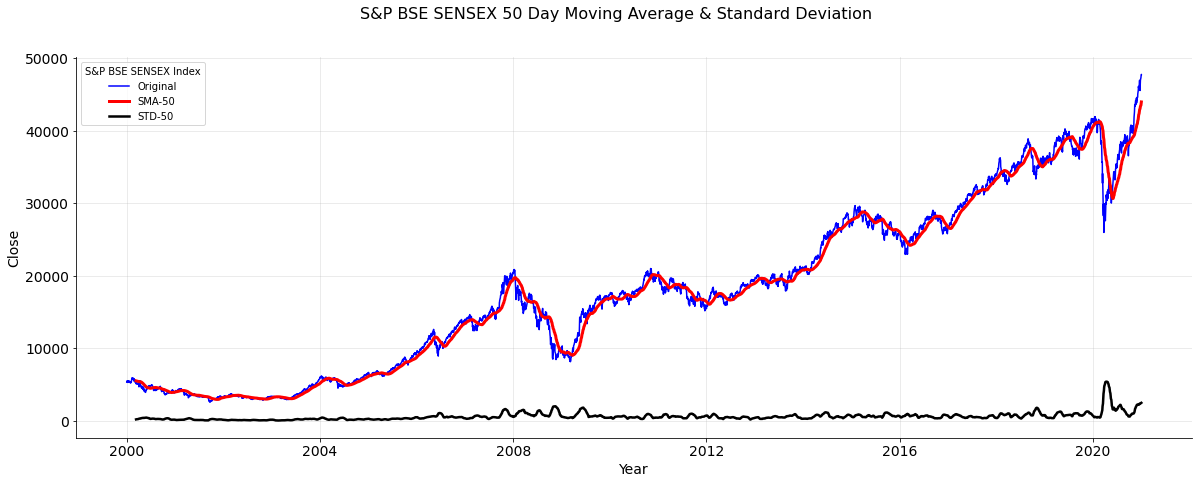
\includegraphics[width = 0.50 \textwidth]{images/SENSEX-Line-Plot.png}
	\caption{S\&P BSE SENSEX Line Plot}
	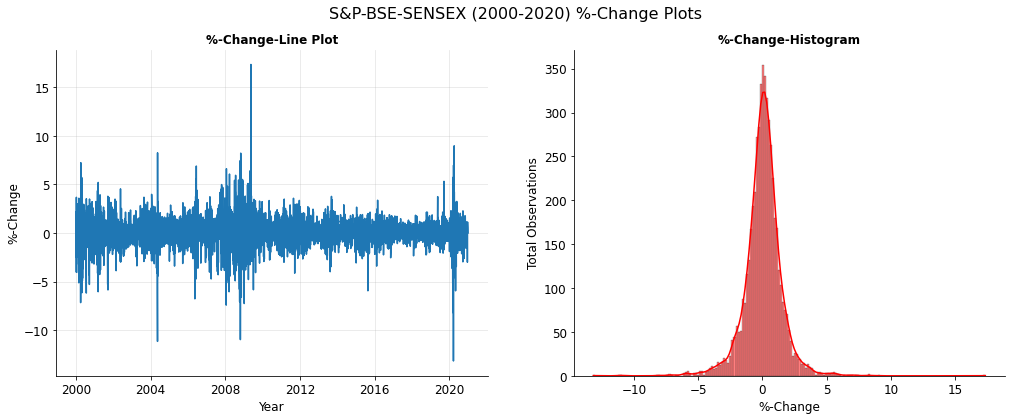
\includegraphics[width = 0.50 \textwidth]{images/SENSEX 2000-2020 Change Plot.png}
	\caption{S\&P BSE SENSEX \%-Change Plots.}
	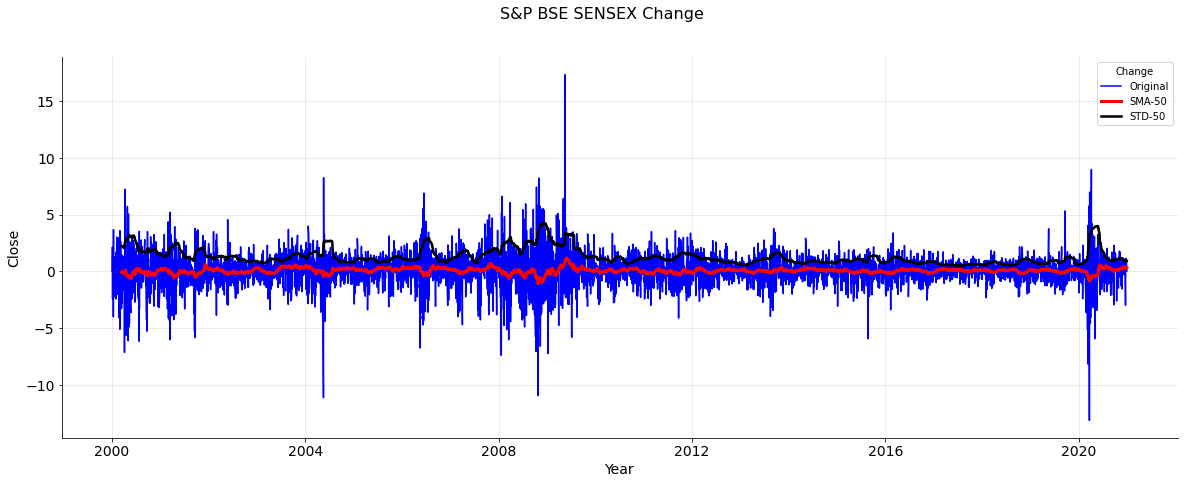
\includegraphics[width = 0.50 \textwidth]{images/BSE SENSEX White Noise Part.png}
	\caption{S\&P BSE SENSEX \%-Change (White Noise Process).}
\end{figure}
	
From Fig.1 you can see clearly that their is a  trend component present in the time series data and also its statistical properties like mean ($\mu$), standard deviation ($\sigma$) and variance ($s$) are dependent on time.
From Fig. 2 you can clearly observe that the \%-Change plot resembles with the white noise process and as the first difference of the given timeseries data (Fig. 3) is a white noise as mean ($\mu \approx 0$) and standard deviation ($\sigma$) is constant implies that the underlying time series data i.e. S\&P BSE SENSEX is a Random Walk process.
A process is a Random Walk process if every value recorded in the series is a result of a random event.
	
Random Walk Process Equations:  $$(i)\; P_{t} = P_{t - 1} + \epsilon_{t}$$
$$ (ii)\; P_{t} = d + P_{t - 1} + \epsilon_{t}$$
$$ (iii)\; P_{t} = P_{0} + dt + \sum_{t = 1}^{n} \epsilon_{t} $$
where   $P_{t} = $ Value of underlying series at time $t$. \\
$P_{t - 1} = $  Value of underlying series at time $t - 1$. \\
$d = $ Drift (which is just a trend like property for a random walk process i.e.\\ $d > 0 \implies$ Upward trend and $d < 0 \implies$ downward trend).\\
$\epsilon_{t} = $ White Noise or Gaussian White Noise.

\subsection{S\&P-500 Index EDA}
Same inferences were observed during the exploratory data analysis of S\&P-500 Index.
\begin{table}[htbp]
	\caption{Descriptive Statistics of S\&P-500 Close and \%-Change Values.}
	\begin{tabular}{c l l l}
		\textbf{Sr.No} & \textbf{Stats}   & \textbf{Close} & \textbf{\%-Change} \\
		1              & Mean             & 1653.27        & 0.025695           \\
		2              & Median           & 1386.95        & 0.0593618          \\
		3              & Min              & 676.53         & -11.9841           \\
		4              & Max              & 3735.36        & 11.58              \\
		5              & Std. Dev         & 673.836        & 1.25313            \\
		6              & Skewness         & 1.03217        & -0.1538            \\
		7              & Kurtosis         & 0.0629593      & 10.736             \\
		8              & Jarque Bera Test & (938.363, 0.0) & (25339.385, 0.0)   \\
	\end{tabular}
\end{table}
	
As $p-value < 0.05$ for Close and \%-Change value of S\&P-500 index implies that the observations recorded are not normally distributed.
	
\begin{figure}[htbp]
	\centering
	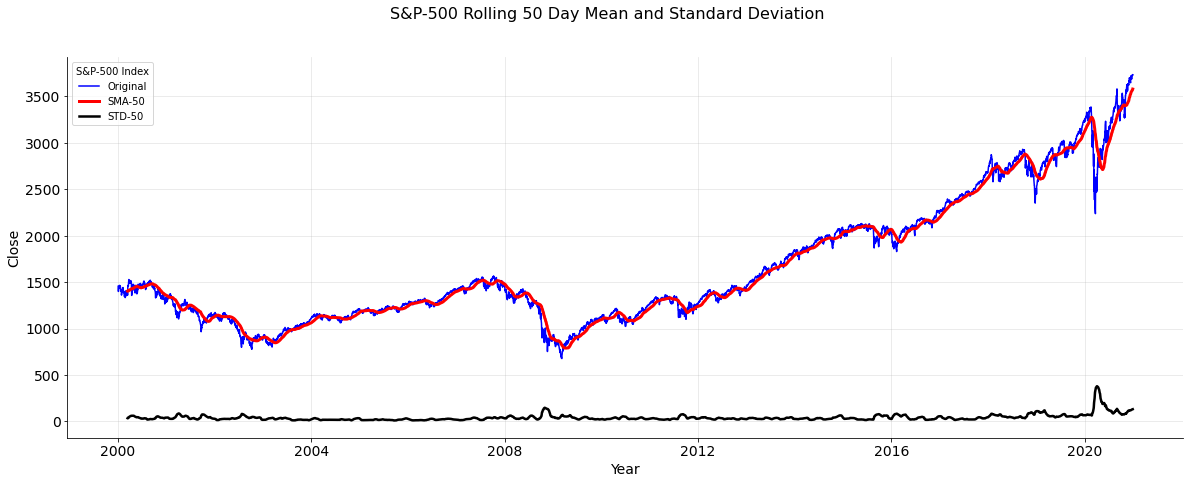
\includegraphics[width = 0.52 \textwidth]{images/S and P-500 Line Plot.png}
	\caption{S\&P-500 Index Line Plot.}
	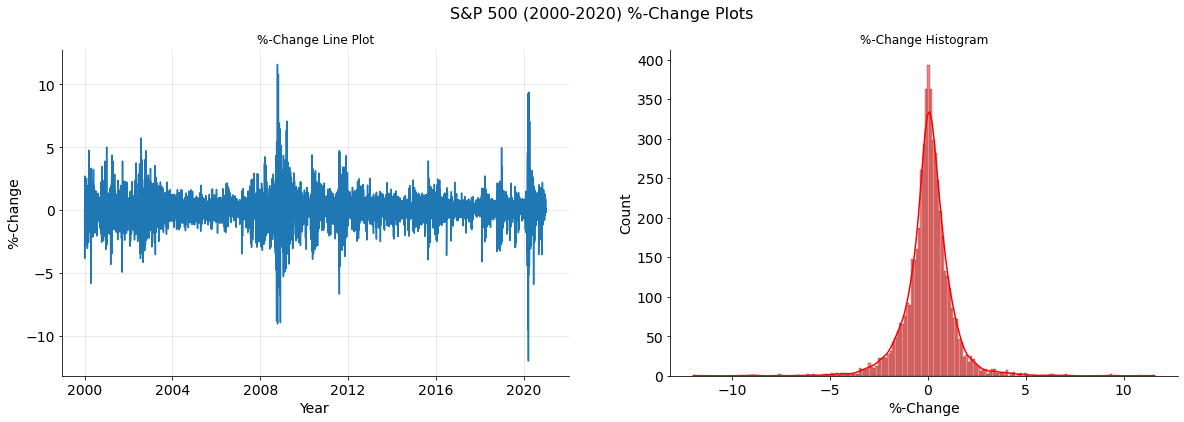
\includegraphics[width = 0.51 \textwidth]{images/S&P-500 Change Plot.png}
	\caption{S\&P-500 \%-Change Plots.}
	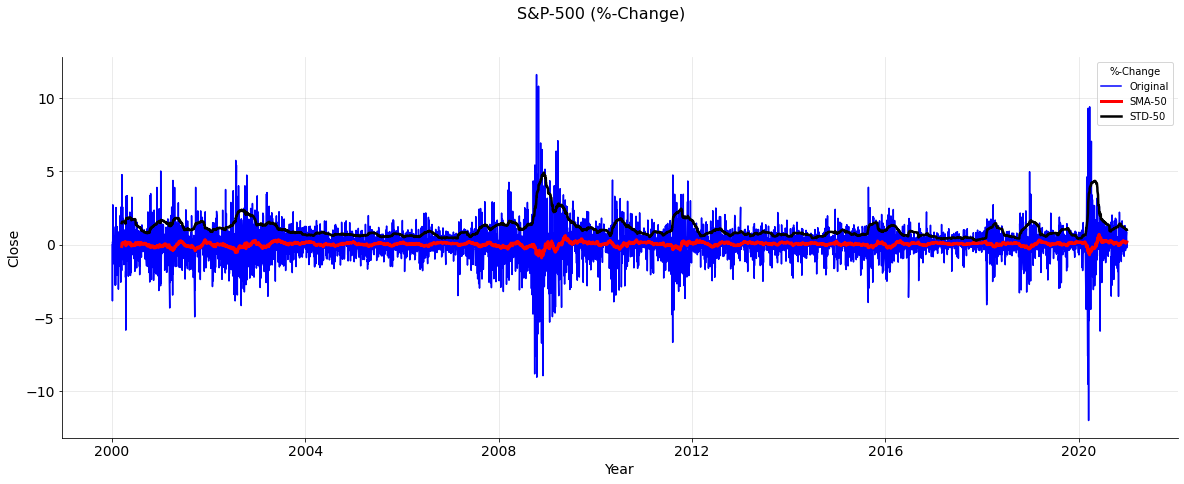
\includegraphics[width = 0.51 \textwidth]{images/S&P-500 White Noise Part.png}
	\caption{S\&P-500 \%-Change (White Noise Process).}
\end{figure}
From Fig.4 you can see clearly that their is a  trend component present in the time series data and also its statistical properties like mean ($\mu$), standard deviation ($\sigma$) and variance ($s$) are dependent on time.
From Fig. 5 you can clearly observe that the \%-Change plot resembles with the white noise process and as the first difference of the given timeseries data (Fig. 6) is a white noise as mean ($\mu \approx 0$) and standard deviation ($\sigma$) is constant implies that the underlying time series data i.e S\&P-500 Index is a Random Walk process.

\subsection{VIX Indexes}
VIX Indexes allows you to measure in real time quantitatively the near term volatility expectations of the market from the perpective of Options market. Fig. 7 shows the India VIX Index and Fig. 8 shows the CBOE VIX Index.
VIX is a trademark of Chicago Board Options Exchange, Incorporated (CBOE) and Standard \& Poor's (S\&P) has granted a license to National Stock Exchange (NSE), with permission from CBOE, to use such mark in the name of the India VIX and for purposes relating to the India VIX.

India VIX is a volatility index computed by NSE based on the order book of NIFTY Options.
For the calculation, the best bid-ask quotes of near and next-month NIFTY options contracts which are traded on the F\&O segment of NSE are used. India VIX depicts the expected market volatility over the next 30 calendar days. Higher the India VIX values, higher the expected volatility and vice-versa.

The CBOE Volatility Index (VIX) quantitatively measure the market's expectations for the relative strength of near-term price changes of the S\&P 500 index (SPX). Because it is derived from the prices of SPX index options with near-term expiration dates, it generates a 30-day forward projection of volatility.

The interesting insights (from Fig. 7 and Fig. 8) to note is that in the FY-2009 and FY-2021, the volatility in the market (both Indian \& United States) are pretty high beacause in the FY-2009, Global Financial Crisis happened due to crash of Mortgage market in United States and in FY-2021 COVID-19 crash happened due to great lockdown and the panic casused by the fear of recession in investors.

\begin{figure}[htbp]
	\centering
	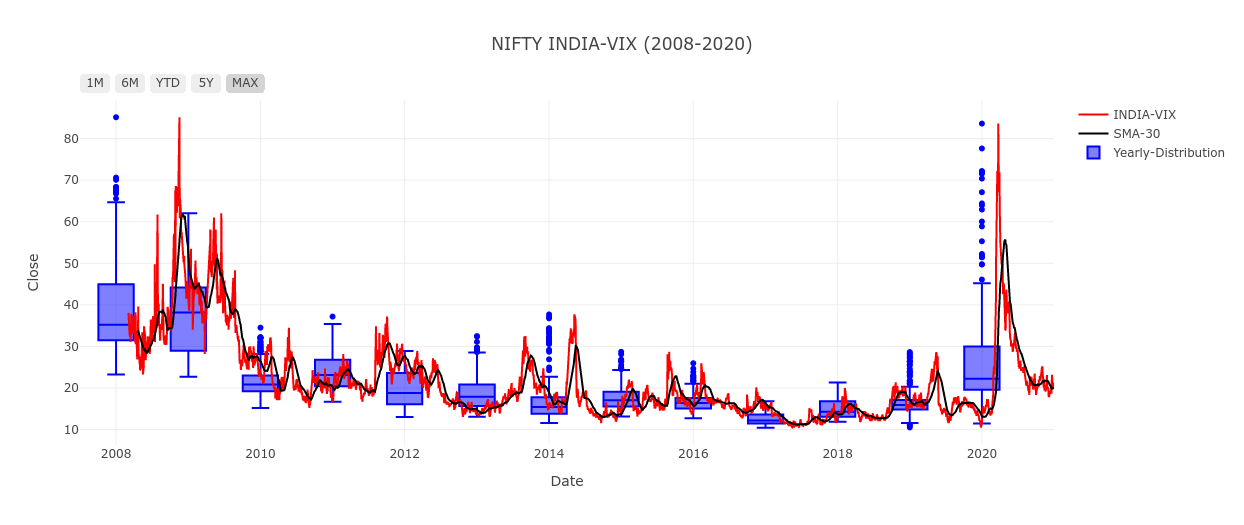
\includegraphics[width = 0.52 \textwidth]{images/INDIA-VIX (2008-2020).png}
	\caption{India VIX Index (2008-2020) Plot.}
	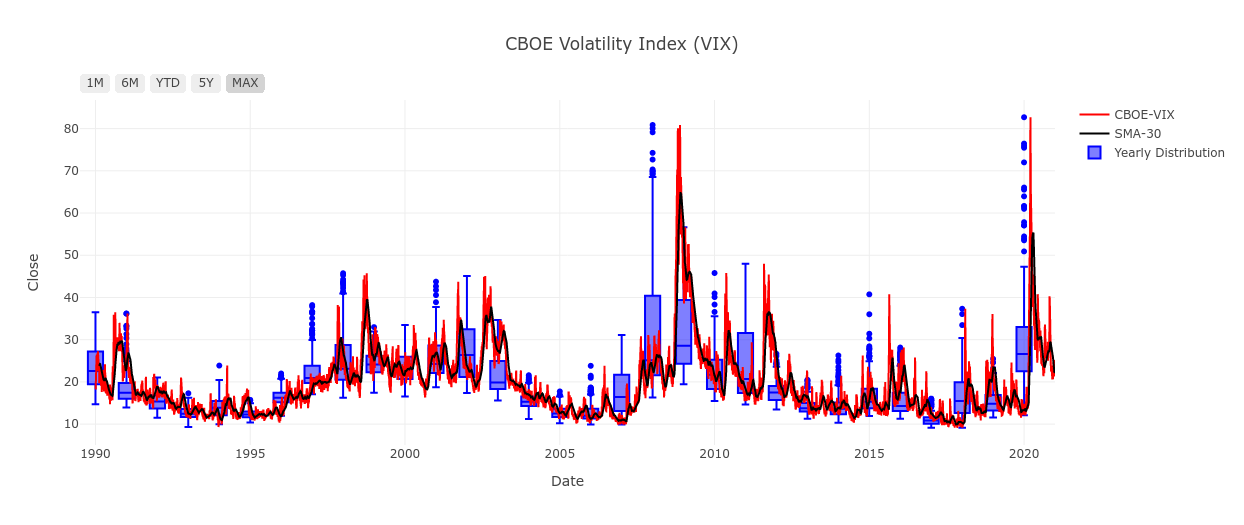
\includegraphics[width = 0.52 \textwidth]{images/CBOE-VIX.png}
	\caption{CBOE VIX Index (1990-2020) Plot.}
\end{figure}

\section{Statistical Tests for Stationarity}
As we have already concluded that the given timeseries data i.e. S\&P BSE SENSEX and S\&P-500 Index are Random Walk Process and all Random Walk Processes are non-stationary in nature.
\subsection{ACF and PACF Plots}
\begin{figure}[htbp]
	\centering
	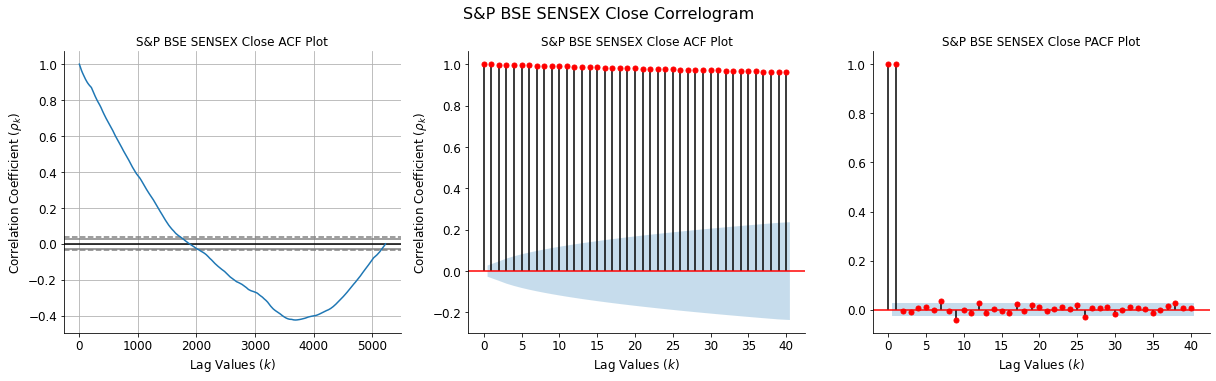
\includegraphics[width = 0.50 \textwidth]{images/SENSEX ACF and PACF Plot.png}
	\caption{S\&P BSE SENSEX ACF and PACF Plots.}
	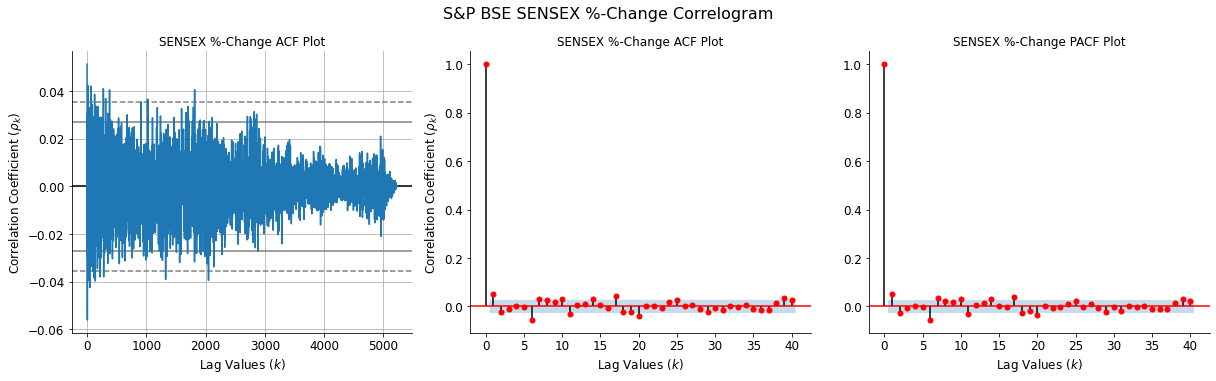
\includegraphics[width = 0.50 \textwidth]{images/SENSEX Change ACF, PACF Plots.png}
	\caption{S\&P BSE SENSEX \%-Change ACF and PACF Plots.}
	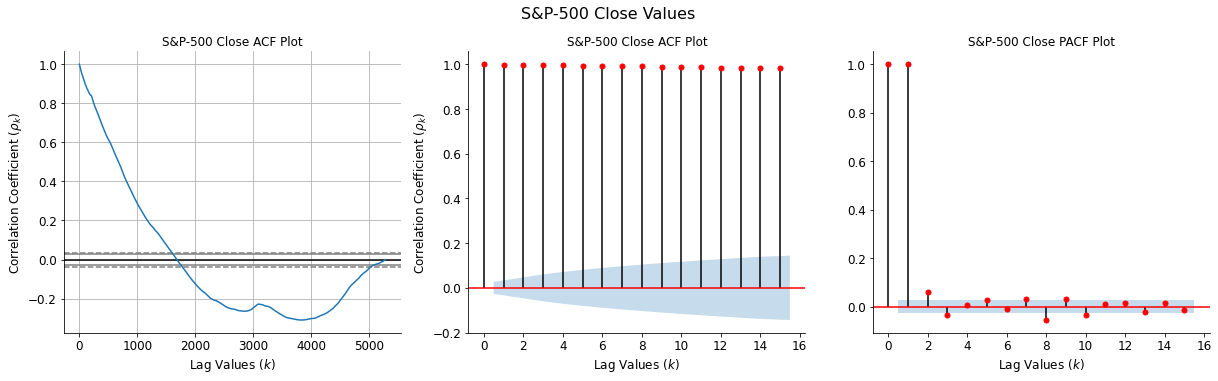
\includegraphics[width = 0.50 \textwidth]{images/S&P-500 ACF, PACF Plots.png}
	\caption{S\&P-500 ACF and PACF Plots.}
	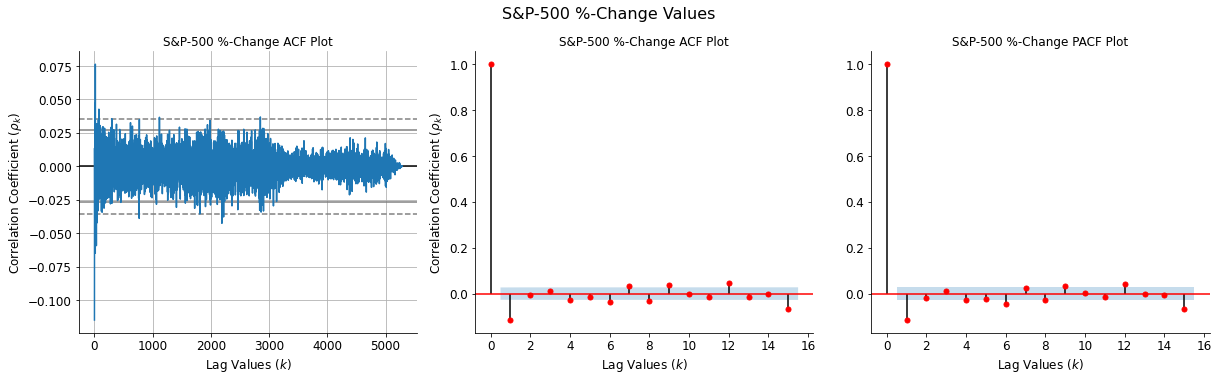
\includegraphics[width = 0.50 \textwidth]{images/S and P-500 Change ACF PACF Plot.png}
	\caption{S\&P-500 \%-Change ACF and PACF Plots.}
\end{figure}
For both the indexes i.e. S\&P BSE SENSEX and S\&P-500 the Close value ACF plot (Fig. 9 and Fig. 11) is unity ($\approx 1$) for short-term lags and its decays down to $0$ at $\approx 1900^{th}$ lag. This is one of the property of the Random Walk Process in which if the number of observations are high with short-term lags ($k$) then we get an autocorrelation ($\rho_{k}$) that is almost unity i.e. we will have extremely high high auto-correlations that does not decreases exponentially as lag increases beacuse the autocorrelation coefficient ($\rho_{k}$) of random walk process is dependent on time and can be derived as follows:
$$\rho_{k}(t) = \frac{Cov(x_{t}, x_{t+k})}{\sqrt{Var(x_{t}) \times Var(x_{t + k})}} = \frac{t\;\sigma^{2}}{\sqrt{t\;\sigma^{2}\times(t + k)\times \sigma^{2}}}$$
Rearranging the terms will give the following equation for autocorrelation coefficient for a random walk process:
$$\rho_{k} = \frac{1}{\sqrt{1 + (k / t)}}$$
You can clearly observe now that $\rho_{k}$ is inversely related to time which explains why $\rho_{k}$ value was unity $\approx 1$ for shorter time lags. 

For both the indexes i.e. S\&P BSE SENSEX and S\&P-500 the \%-Change ACF plot (Fig. 10 and Fig. 12) doesn't show any statistically significant correlation at lags $k$ and $95\%$ of the spikes in ACF plots are in the range of $\pm \frac{2}{\sqrt{T}}$ where $T$ represents the number of observations which means the underlying \%-Change sequence is a white noise process.

\subsection{Augmented Dickey Fuller (ADF) Tests}
Augmented Dickey Fuller (ADF) test is one of the unit root tests to check the stationarity of the timeseries data through hypothesis testing.

$H_{0}$: Given time series data is non-stationarity $\implies$ Time series data has time dependent statistical properties i.e. mean, variance, auto-correlation etc present in it.

$H_{A}:$ Given time series data is stationary $\implies$ Time series data doesn't have any time dependent statisitcal properties present in it. \newline
$p-value \le 0.05$ then we reject the $H_{0}$ otherwise we don't have enough evidence to reject the $H_{0} \implies$ failed to reject $H_{0}.$ \newline
The results of ADF Test performed on both the indexes is shown in the tables.
\begin{table}[htbp]
	\caption{S\&P BSE SENSEX Close Value ADF Test Results.}
	\begin{tabular}{|c|c|c|c|c|}
		\hline
		\textbf{Sr.No} & \textbf{Data} & \textbf{t-statistic} & \textbf{p-value} & \textbf{Verdict}        \\
		\hline
		1              & Close Values  & $0.688133$           & $0.688133$       & Failed to Reject H_{0}. \\
		\hline
	\end{tabular}
\end{table}

As p-value obtained i.e. $0.998199 > 0.05 (\alpha) \implies$ Failed to Reject $H_{0} \implies$ S\&P BSE SENSEX Close values is \textbf{non-stationary} (Table. IV).

\begin{table}[htbp]
	\caption{S\&P BSE SENSEX \%-Change Values ADF Test Results.}
	\centering
	\begin{tabular}{|c|c|c|c|c|}
		\hline
		\textbf{Sr.No} & \textbf{Data}    & \textbf{t-statistic} & \textbf{p-value}        & \textbf{Verdict} \\
		\hline
		1              & \%-Change Values & $-16.081$            & $5.390 \times 10^{-29}$ & Reject H_{0}.    \\
		\hline
	\end{tabular}
\end{table}
As p-value obtained i.e. $5.389647 \times 10^{-27} << 0.05 (\alpha) \implies$ Reject the $H_{0} \implies$ S\&P BSE SENSEX \%-Change values is \textbf{stationary} (Table. V).

\begin{table}[htbp]
	\caption{S\&P-500 Close Value ADF Test Results.}
	\begin{tabular}{|c|c|c|c|c|}
		\hline
		\textbf{Sr.No} & \textbf{Data} & \textbf{t-statistic} & \textbf{p-value} & \textbf{Verdict}        \\
		\hline
		1              & Close Values  & $1.631761$           & $0.99795$        & Failed to Reject H_{0}. \\
		\hline
	\end{tabular}
\end{table}
As p-value obtained i.e. $0.99795 > 0.05 (\alpha) \implies$ Failed to Reject $H_{0} \implies$ S\&P-500 Close values is \textbf{non-stationary} (Table. VI).
	
\begin{table}[htbp]
	\centering
	\caption{S\&P-500 \%-Change Values ADF Test Results.}
	\begin{tabular}{|c|c|c|c|c|}
		\hline
		\textbf{Sr.No} & \textbf{Data}    & \textbf{t-statistic} & \textbf{p-value}        & \textbf{Verdict} \\
		\hline
		1              & \%-Change Values & $-13.742$            & $1.095 \times 10^{-25}$ & Reject H_{0}.    \\
		\hline
	\end{tabular}
\end{table}
As p-value obtained i.e. $1.094051 \times 10^{-25} << 0.05 (\alpha) \implies$ Reject the $H_{0} \implies$ S\&P-500 \%-Change values is \textbf{stationary} (Table. VII).

\section{Estimating Parameters of Models}
The model used is SARIMA but as we are also exposing the SARIMA model to exogenous features i.e. those features which are not used to fit the model but have an influence on the model forecast. Hence the model used is SARIMAX where X is for exogeneous features presence.

For Prophet library based predictions we don't need to estimate parameters because the library has abstracted that process.

\subsection{S\&P BSE SENSEX Index}
Estimated hyperparameters of SARIMAX $(p, d, q) \times (P, D, Q, M)$ are: \textbf{SARIMAX $(2, 0, 1) \times (2, 0, 0, 7)$} with an AIC $=63798.806$.

\subsection{S\&P-500 Index}
Estimated hyperparameters of SARIMAX$(p, d, q) \times (P, D, Q, M)$ are: \textbf{SARIMAX} $(5, 1, 1) \times (2, 0, 1, 7)$ with an AIC=$35701.260$.

\section{Validation For Actual and Forecasted Values}
\subsection{S\&P BSE SENSEX Index}
The following graphs shows the performance of the model (SARIMAX and Prophet) on validation data of S\&P BSE SENSEX.
\begin{figure}[htbp]
	\centering
	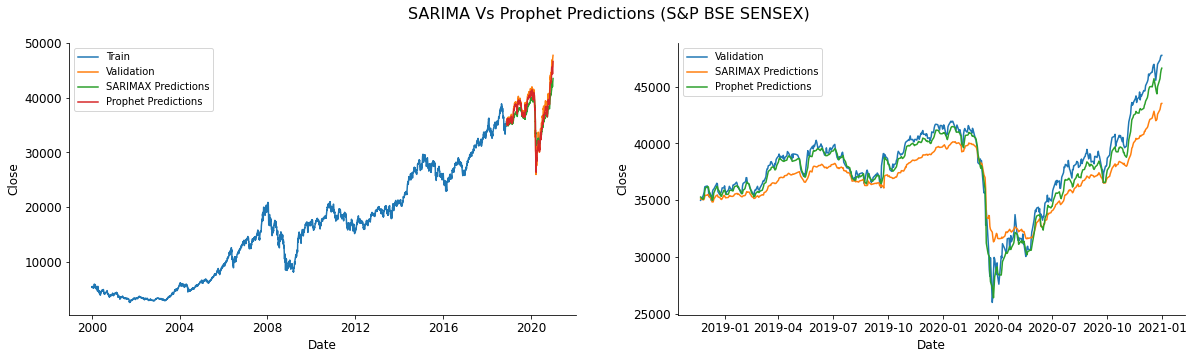
\includegraphics[width = 0.50 \textwidth]{images/SARIMAX-Prophet-SENSEX-Predictions.png}
	\caption{SARIMAX and Prophet Model Predictions on Validation Data for S\&P BSE SENSEX.}
\end{figure}
\begin{table}[htbp]
	\centering
	\caption{SARIMAX and Prophet Error Metric Values.}
	\begin{tabular}{c c c c c c}
		\textbf{Model} & \textbf{MAE} & \textbf{MSE}          & \textbf{RMSE} & \textbf{R2-Score} & \textbf{MAPE} \\
		SARIMAX        & 1553.135     & $3.386 \times 10^{6}$ & 1839.904      & 0.731307          & $4.05 \%$     \\
		Prophet        & 611.323      & $5.998 \times 10^{5}$ & 774.435       & 0.953             & $1.60\%$      \\
	\end{tabular}
\end{table}
\subsection{S\&P-500 Index}
The following graphs shows the performance of the model (SARIMAX and Prophet) on validation data of S\&P-500 Index.

\begin{figure}[htbp]
	\centering
	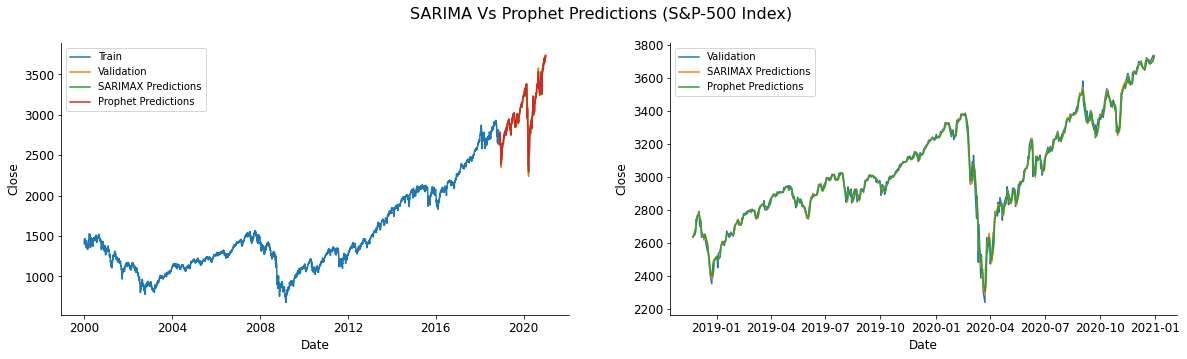
\includegraphics[width = 0.50 \textwidth]{images/SARIMAX-Prophet-S&P-500-Predictions.png}
	\caption{SARIMAX and Prophet Model Predictions on Validation Data for S\&P-500.}
\end{figure}
\begin{table}[htbp]
	\centering
	\caption{SARIMAX and Prophet Error Metric Values.}
	\begin{tabular}{c c c c c c}
		\textbf{Model} & \textbf{MAE} & \textbf{MSE} & \textbf{RMSE} & \textbf{R2-Score} & \textbf{MAPE} \\
		SARIMAX        & 18.189       & 755.416      & 27.484822     & 0.991685          & $0.62 \%$     \\
		Prophet        & 18.452       & 770.787      & 27.764        & 0.991516          & $0.63\%$      \\
	\end{tabular}
\end{table}

\section{Findings from the Study}
The volatility which was obeserved during the Global Financial Crisis of 2008, the same kind of volatility was observed in the COVID Crash of 2020 in both the markets i.e. USA and India.

The markets independent of geography not only tells us the sentiment of the investor in short-term but also gives us an idea about what are the variables which plays a major role like budget annoucements, stimulus plans, FDIs etc to move the market in either directions, but in long term only those stocks/equities/securities performed well which represents high quality businesses.

Both the markets i.e. Developed \& Emerging markets have rebounded quickly i.e. in approximately 7 months after the COVID-19 crash which itself is a thing to discuss because normally it takes atleast 2 years for the markets to recover to its early highs.

\section{Conclusions}
In this analysis, \textbf{SARIMAX$(2, 0, 0) \times (2, 0, 0, 7)$} for S\&P BSE SENSEX and \textbf{SARIMAX$(5, 1, 1) \times (2, 0, 1, 7)$} for S\&P-500 yielded a highly accurate results with a MAPE of $4.05\%$ and $0.61\%$.

Prophet has performed better than both the ARIMA models when forecasting S\&P BSE SENSEX and S\&P-500 with MAPE of $1.06\%$ and $0.62\%$.

This model can be used as a techinical indicator of what values the indexes would take in short term in order manage the portfolios to maximize the profits in the market.

\section{Future Work}
In addition to forecasting the closing price, it will also be more strategic if we can also forecast the $\beta$ value i.e. measure of risk with respect to benchmark indices or broader market indices \cite{b3}.

Adding more exogenous variables like P/E ratio, P/B ratio, Market Capitalisation etc as external features in the dataset can help in building a more robust model for forecasting.

\begin{thebibliography}{00}
	\bibitem{b1} Fama, Eugene F. “Efficient Capital Markets: A Review of Empirical Work.” Journal of Finance 25, no. 2 (1970): 383–417.
	
	\bibitem{b2} Madhavi Latha Challa \& Venkataramanaiah Malepati \& Siva Nageswara Rao Kolusu, 2020. "S\&P BSE Sensex and S\&P BSE IT return forecasting using ARIMA," Financial Innovation, Springer, Southwestern University of Finance and Economics, vol. 6(1), pages 1-19, December.
	
	\bibitem{b3} Challa, M.L., Malepati, V. \& Kolusu , S.N.R. Forecasting risk using auto regressive integrated moving average approach: an evidence from S\&P BSE Sensex. Financ Innov 4, 24 (2018). https://doi.org/10.1186/s40854-018-0107-z
\end{thebibliography}

\appendix
\subsection{Appendix-I}
For interactive plots, source codes and implementation please refer:\newline
\textbf{GitHub Link:} \href{https://github.com/strikersps/Forecasting-BSE-SENSEX-and-S-and-P-500-Using-ARIMA-and-Prophet}{https://github.com/strikersps/Forecasting-BSE-SENSEX-and-S-and-P-500-Using-ARIMA-and-Prophet} \newline
\end{document}